\documentclass{article}

\usepackage[T1]{fontenc}
\usepackage[polish]{babel}
\usepackage[utf8]{inputenc}
\usepackage{float}
\usepackage{graphicx}
\usepackage{amsmath}
\usepackage{siunitx}
\oddsidemargin 0pt
\evensidemargin 0pt
\marginparwidth 40pt
\marginparsep 10pt
\topmargin -20pt
\headsep 10pt
\textheight 8.7in
\textwidth 6.65in
\linespread{1.2}

\title{Sprawozdanie z Laboratorium 3. \\ \large Ciepło Właściwe }
\author{Piotr Lewandowski \and Dymitr Lubczyk \and Krzysztof Tabeau }
\date{\today}

\begin{document}
\maketitle
\clearpage
\section{Część teoretyczna}
\subsection{Wstęp}
W poniższym sprawozdaniu zamierzamy przedstawić wyniki dwóch eksperymentów mających na celu wyznaczenie ciepła właściwego kalorymetru oraz ciepła topnienia lodu. W poniższym sprawozdaniu będziemy się posługiwali takimi pojęciami jak  bilans cieplny, ciepło, ciepło właściwe, kalorymetr czy temperatura, więc pokrótce pozwolimy sobie je przedstawić:
\begin{itemize}
\item Bilans cieplny - jest to przełożenie zasady zachowania energii do opisu wymiany ciepła w procesach termodynamicznych.
\item Ciepło - rozumiemy przez to zmianę energii wewnętrznej, podczas jakiegoś procesu termodynamicznego.
\item Ciepło właściwe - jest to właściwość substancji mówiąca o tym jak wiele energii musimy dostarczyć, aby zwiększyć jej temperaturę, podawane dla zmiany ciała o masie $1 kg$ przy zmianie o $1K$.
\item Kalorymetr - jest to przyrząd pomiarowy wykorzystywany do mierzenia wymiany ciepła w procesach termodynamicznych.
\item Temperatura - rozumiemy przez to miarę średniej energii kinetycznej cząstek w danym ciele.
\end{itemize}
\subsection{Opis układów doświadczalnych}
W doświadczeniu mającym na celu wyznaczenie ciepła właściwego kalorymetru będziemy używali kalorymetru, wagi mającej na celu zmierzenie masy dolewanej wody, termometru służącego do określenia temperatury dolewanej wody oraz oczywiście wody. Przebieg doświadczenia jest następujący, do kalorymetru z wodą będącego w stanie równowagi, dolewamy wody o temperaturze wyższej niż tej w kalorymetrze i z bilansu cieplnego otrzymujemy następujące równanie
\begin{equation}
    m_{2}\cdot c_{w}\cdot (T_{2}-T)=m_{1}\cdot c_{w}\cdot (T-T_{k})+m_{k}\cdot c_{k}\cdot (T-T_{k})
\end{equation}
które przekształcamy do
\begin{equation}
        c_{k}=\frac{c_{w}\cdot((m_{2}\cdot (T_{2}-T)+m_{1}\cdot (T-T_{k}))}{m_{k}\cdot (T-T_{k})}
\end{equation}
gdzie
\begin{itemize}
\item$m_{1}$ - masa wody w kalorymetrze przed dolaniem
\item$m_{2}$ - masa wody dolewanej
\item$m_{k}$ - masa kalorymetru
\item$c_{k}$ - ciepło właściwe kalorymetru
\item$c_{w}$ - ciepło właściwe wody
\item$T_{k}$ - temperatura kalorymetru oraz wody w nim zawartej przed dolaniem
\item$T_{2}$ - temperatura wody dolewanej
\item$T$ - temperatura układu po ustaleniu się stanu równowagi po dolaniu
\end{itemize}
zamierzamy wykonać pięć pomiarów, uśrednić otrzymane wyniki oraz obliczyć niepewności pomiarowe typu B.\\\\
W drugiej części eksperymentu zamierzamy wyznaczyć ciepło topnienia lodu. Procedura będzie bardzo podobna do powyższej, z wyjątkiem tego, że zamiast wrzucać kolejne porcje wody, do kalorymetru będzie wrzucali kostki lodu. Podobnie jak powyżej skorzystamy z bilansu cieplnego otrzymując

\begin{equation}
     m_l\cdot q_l+m_l\cdot c_{w}\cdot T=m_{1}\cdot c_{w}\cdot (T_{k}-T)+m_{k}\cdot c_{k}\cdot (T_{k}-T)
\end{equation}
co przekształcamy do 
\begin{equation}
    q_l=\frac{ (T_{k}-T)\cdot (m_{1}\cdot c_{w}+m_{k}\cdot c_{k})}{m_l}-c_w\cdot T
\end{equation}
gdzie 
\begin{itemize}
\item$m_{l}$ - masa wrzucanego lodu
\item$q_l$ - ciepło topnienia lodu 
\end{itemize}
pozostałe oznaczenia są analogiczne do tych z doświadczenia, w którym wyznaczaliśmy ciepło właściwe kalorymetru

\clearpage

\section{Część doświadczalna}
\subsection{Wykonane pomiary}
Pomiary wykonane w doświadczeniu, w którym wyznaczaliśmy ciepło właściwe kalorymetru o masie 765g
\begin{table}[h!]
\centering
\begin{tabular}{|l|l|l|l|l|l|}
\hline
$T_{k} [C]$ & $m_{1} [kg]$ &  $T_{2}[C]$ &  $m_{2} [kg]$ & $T [C]$      &$c_{k} [\frac{J}{kg\cdot K}]$                \\ \hline
20          & 0,5       & 40                & 0,3             &26,22        &900.19                 \\ 
26,22       & 0,8       & 50                & 0,3             &31,86        &901.63               \\ 
31,86       & 1,1       & 60                & 0,3             &37,26        &893.10                 \\ 
37,26       & 1,4       & 70                & 0,3             &42,52        &914.79              \\ 
42,52       & 1,7       & 90                & 0,3             &49.10        &900.80             \\ \hline
\end{tabular}
\caption{Zmiany stanu kalorymetru wraz z jego ciepłami właściwymi}
\end{table}

Pomiary wykonane w doświadczeniu mającym na celu wyznaczenie ciepła topnienia lodu, kolejne pomiary uzyskiwaliśmy po przez wrzucanie kostek lodu do kalorymetru z woda.
\begin{table}[h!]
\centering
\begin{tabular}{|l|l|l|l|l|}
\hline
$m_w [kg]$ & $m_l [kg]$ & $T_k [C]$ & $T [C]$ & $q_l[\frac{J}{kg}]$ \\ \hline
1      & 0.0243 & 90      & 86.531              & 333657        \\
1.0243 & 0.0243 & 86.531  & 83.201              & 333643           \\
1.0486 & 0.0243 & 83.201  & 80.0018             & 333632      \\
1.0729 & 0.0243 & 80.0018 & 76.9258             & 333631       \\
1.0972 & 0.0243 & 76.9258 & 73.9661             & 333611        \\
1.1215 & 0.0243 & 73.9661 & 71.1161             & 333621      \\
1.1458 & 0.0243 & 71.1161 & 68.3699             & 333611      \\
1.1701 & 0.0243 & 68.3699 & 65.7219             & 333608      \\
1.1944 & 0.0243 & 65.7219 & 63.167              & 333587       \\
1.2187 & 0.0243 & 63.167  & 60.7003             & 333586       \\
1.243  & 0.0243 & 60.7003 & 58.3173             & 333587    \\
1.2673 & 0.0243 & 58.3173 & 56.0138             & 333591\\
1.2916 & 0.0243 & 56.0138 & 53.786              & 333566\\
1.3159 & 0.0243 & 53.786  & 51.6301             & 333576\\
1.3402 & 0.0243 & 51.6301 & 49.5427             & 333578 \\
1.3645 & 0.0243 & 49.5427 & 47.5206             & 333577 \\
1.3888 & 0.0243 & 47.5206 & 45.5609             & 333544 \\
1.4131 & 0.0243 & 45.5609 & 43.6606             & 333555\\
1.4374 & 0.0243 & 43.6606 & 41.8171             & 333549\\
1.4617 & 0.0243 & 41.8171 & 40.0278             & 333567\\
\hline
\end{tabular}
\caption{Temperatura wody w zależności od liczby kostek}
\end{table}

\clearpage
\subsection{Opracowanie wyników}
W celu określania niepewności pomiarowej ciepła właściwego kalorymetru posłużyliśmy się niepewnością pomiarową typu B. Niepewność pomiarowa kalorymetru wyraża się wzorem
$$
    u(c_{k})= \sqrt{  
     \frac{\partial c_k}{\partial m_{2} } u^2_b(m_{2}) +
     \frac{\partial c_k}{\partial m_{1} } u^2_b(m_{1}) +
     \frac{\partial c_k}{\partial T } u^2_b(T) + 
     \frac{\partial c_k}{\partial T_{k} } u^2_b(T_{k}) +
     \frac{\partial c_k}{\partial T_{2} } u^2_b(T_{2})
    }   
$$
gdzie
\begin{gather*}
    \frac{\partial c_k}{\partial m_{2} } = \frac{c_{w}}{m_k} \left(  \frac{T_2 - T}{T - T_k} \right) \\
    \frac{\partial c_k}{\partial m_{1} } = \frac{c_{w}}{m_k} \\
    \frac{\partial c_k}{\partial T } = \frac{c_{w}}{m_k} \left(  \frac{T_k - T_2}{(T - T_k)^2} \right) \\
    \frac{\partial c_k}{\partial T_{k} } = \frac{c_{w}}{m_k} \left(  \frac{T_2 - T}{(T - T_k)^2} \right) \\
    \frac{\partial c_k}{\partial T_2 } = \frac{c_{w}}{m_k} \frac{m_2}{T - T_k}
\end{gather*}
\\\\Co prowadzi do ostatecznego rezultatu
$$
c_k=(902\pm 16)\frac{J}{kg \cdot K}
$$
    \begin{figure}[h!]
    \centerline{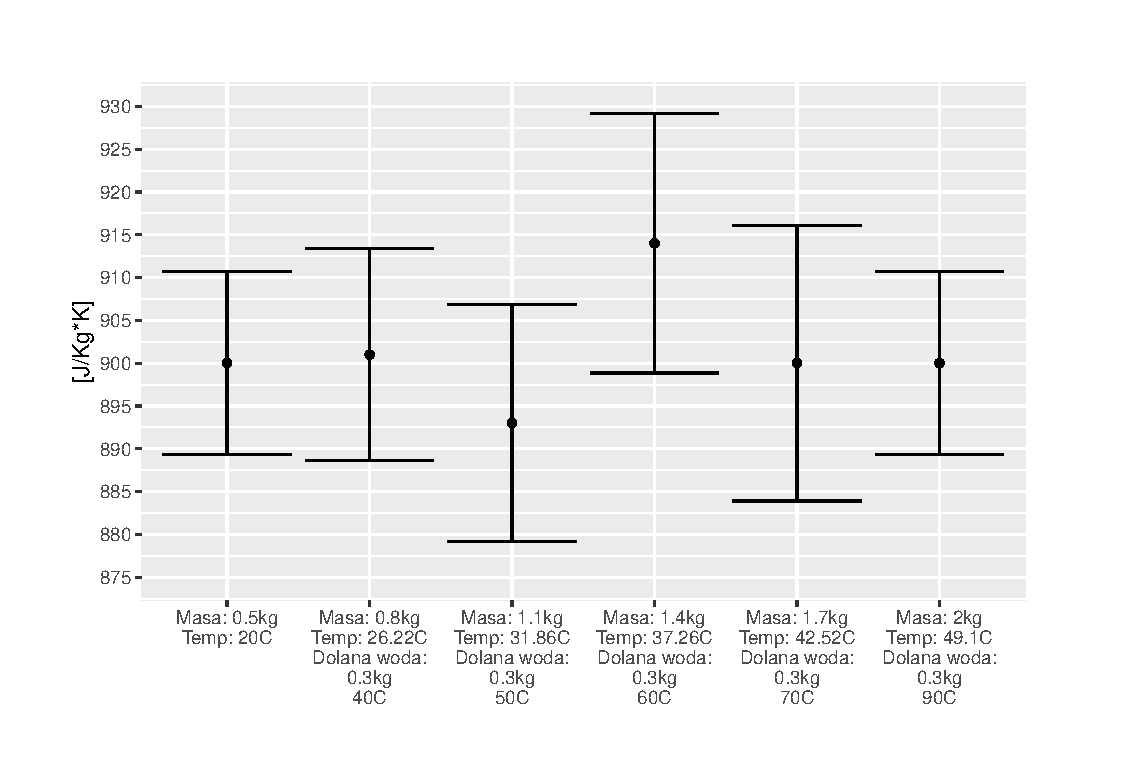
\includegraphics[scale=0.65]{kalorymetr}}
    \caption{Ciepło właściwe kalorymetru}
    \end{figure}
\clearpage
W drugim doświadczeniu wyznaczaliśmy ciepło topnienia lodu, poniżej przedstawiamy wzór na jego niepewność pomiarową 
$$
    u(q_l) = \sqrt{
    \frac{\partial q_l}{\partial m_{1} } u^2_b(m_{1})+ 
    \frac{\partial q_l}{\partial c_{k} }  u^2_b(c_k) +
    \frac{\partial q_l}{\partial T } u^2_b(T) +
    \frac{\partial q_l}{\partial T_{k} } u^2_b(T_{k})
    }
$$
gdzie obliczone przez nas pochodne cząstkowe, wyrażają się wzorami
\begin{gather*}
    \frac{\partial q_l}{\partial m_{1} } = \frac{c_{w} (T_{k} - T) }{m_l}  \\
    \frac{\partial q_l}{\partial c_{k} } = \frac{m_k (T_{k} - T) }{m_l} - T \\
    \frac{\partial q_l}{\partial T } = - \frac{ m_{1} c_{w} + m_k c_{k} }{m_l} - c_w \\
    \frac{\partial q_l}{\partial T_{k} } = \frac{ m_{1} c_{w} + m_k c_{k} }{m_l}
\end{gather*}
\\Co ostatecznie daje
$$
q_l=(333594\pm 102)\frac{J}{kg}
$$

\begin{figure}[h!]
\centerline{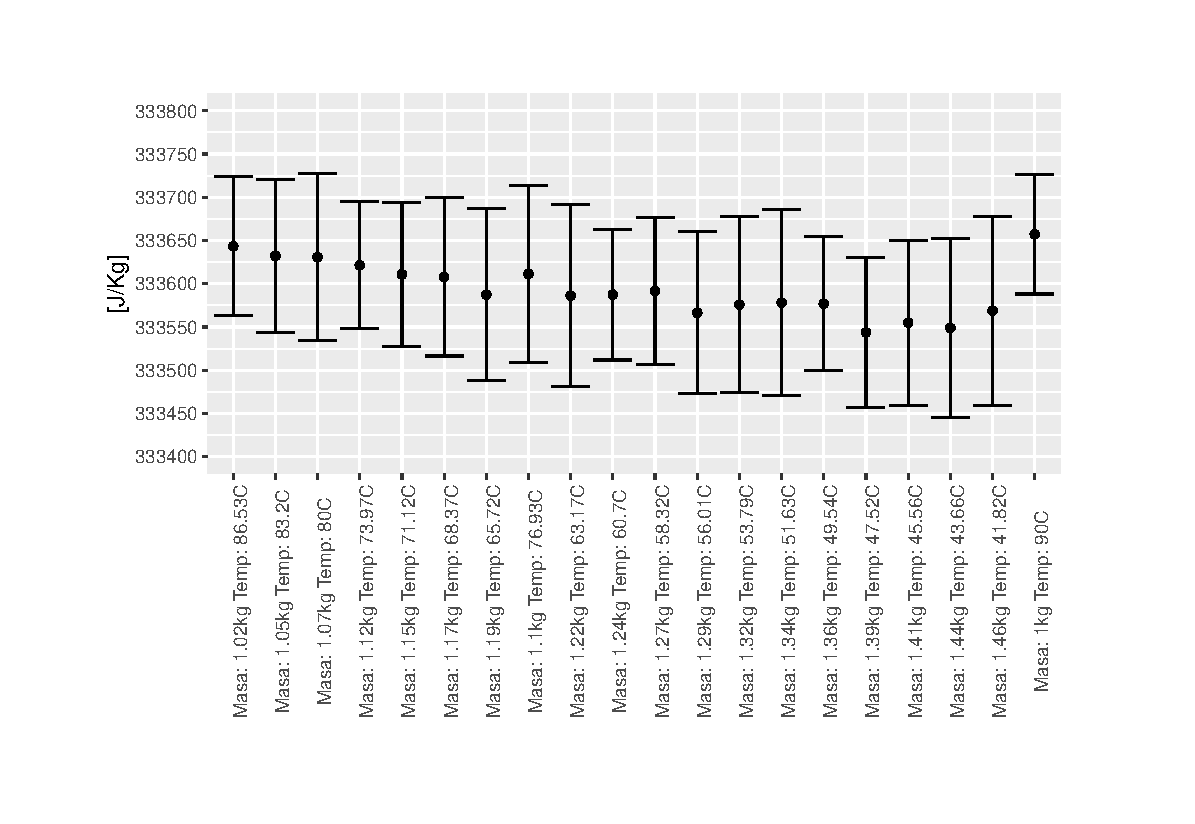
\includegraphics[scale=0.7]{lod}}
\caption{Ciepło topnienia lodu}
\end{figure}

\pagebreak

\subsection{Podsumowanie}
Uważam, że efekt doświadczenia jest bardzo satysfakcjonujący, ponieważ udało się wyznaczyć ciepło topnienia lodu z niebywała dokładnością, jednakże ma on wiele problemów, przede wszystkim doświadczenie zostało przeprowadzone na podstawie wyników otrzymanych z symulacji, a nie zebranych podczas faktycznego doświadczenia, dodatkowo liczba zebranych próbek jest dość mala, co jest kolejnym brakiem. Uważam, ze gdyby  było to możliwie, bardzo ciekawym byłoby odtworzenie tego doświadczenia w fizycznym laboratorium. Tym bardziej, że jest to bardzo podstawowe doświadczenie fizyczne i uważam, że rozwija zdolności, które powinny być w elementarzu każdego inżyniera.


\end{document}
